\documentclass {article}

\usepackage {amsthm}
\usepackage {amssymb}
\usepackage {amsmath}
\usepackage {fancyhdr}
\usepackage {graphics}
\usepackage {multicol}

\usepackage[margin=1.15in]{geometry}

\newenvironment{prob}[2][]{\begin{trivlist}
\item[\hskip \labelsep {\bfseries #1}\hskip \labelsep {\bfseries #2.}]}{\end{trivlist}}

\newcommand {\fspace}{\vspace {\fill}}
\newcommand {\blank} [1] {\underline{\hspace{#1cm}}}

\thispagestyle {fancy}
\lhead {\textbf{Name:}}
\chead {MTH 103 \\ Section 65}
\rhead {Quiz 3 \\ 2/11/14}

\begin {document}

\ \\ \\ \relax
\noindent Make sure to \textbf{clearly show all your work} (except on number 1). Grades will be based on your intermediate steps
as well as the final answer.

\vspace {1cm}

\begin {prob}{1} (4 points)
    In the blanks to the right of each inequality in parts $(i) \sim (iv)$, choose the diagram below ($a,b,c$, or $d$)
    which depicts the solution set.
    \begin {multicols}{2}
        \[ \begin {array}{rcc}
            (i)   &  x - a  > r & \underline{\hspace{2cm}} \\ [3ex]
            (ii)  & x - a   < r & \underline{\hspace{2cm}} \\ [3ex]
            (iii) & |x - a| > r & \underline{\hspace{2cm}} \\ [3ex]
            (iv)  & |x - a| < r & \underline{\hspace{2cm}} 
        \end {array} \]

        \vfill

        \begin {center}
            \scalebox{0.3}{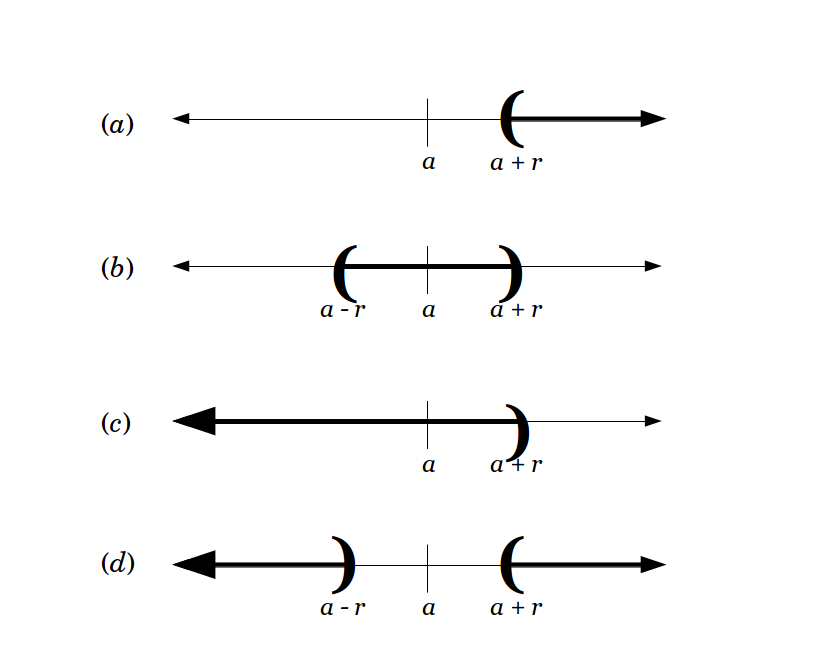
\includegraphics{num_line}}
        \end {center}
    \end {multicols}
\end {prob}

\begin {prob}{2} (4 points)
    Solve the following polynomial inequality and write the solution set \textbf{in interval notation}.
    \[ 2x - 3 \leq 7x + 5 \]
\end {prob}

\vfill

\begin {prob}{3} (4 points)
    Find all solutions to the equation:
    \[ \left| 2x - 6 \right| + 1 = 9 \]
\end {prob}

\vfill

\newpage

\begin {prob}{4} (4 points)
    Solve the following rational inequality and write the solution set \textbf{in interval notation}.
    \[ \frac{2 - x}{3x + 1} > 0 \]
\end {prob}


\vfill

\begin {prob}{5} (4 points)
    Solve the following inequality and write the solution set \textbf{in interval notation}:
    \[ \left| 5x - 1 \right| < 2 \]
\end {prob}

\vfill

\newpage

\section* {Solutions}

\begin {prob}{1} \ \\ \\ \relax
    \begin {tabular}{rl}
        $(i)$   & $(a)$ \\
        $(ii)$  & $(c)$ \\
        $(iii)$ & $(d)$ \\
        $(iv)$  & $(b)$ 
    \end {tabular}
\end {prob}

\vspace {1cm}

\begin {prob}{2}
    Solve the following polynomial inequality and write the solution set \textbf{in interval notation}.
    \[ 2x - 3 \leq 7x + 5 \]
\end {prob}

\begin {align*}
    2x - 3 &\leq 7x + 5 \\
    2x - 8 &\leq 7x \tag{subtract 5} \\
    -8     &\leq 5x \tag{subtract $2x$} \\
    -\frac{8}{5} &\leq x \tag{divide}
\end {align*}
The solution set is described by $x \geq -\frac{8}{5}$, which in interval notation is $\left[ -\frac{8}{5}, \infty \right)$.

\vspace {1cm}

\begin {prob}{3}
    Find all solutions to the equation:
    \[ \left| 2x - 6 \right| + 1 = 9 \]
\end {prob}

Begin by isolating the absolute value expression. So subtract 1 to get
\[ |2x - 6| = 8 \]

Now we just solve the two equations $2x-6=8$ and $2x-6 = -8$:
\[ 
    \begin{array}{ccc|ccc}
        2x - 6 &=& 8  &  2x - 6 &=& -8 \\
        2x     &=& 14 &  2x     &=& -2 \\
        x      &=& 7  &  x      &=& -1
    \end{array}
\]
The only two solutions are then $x=7$ and $x=-1$.

\newpage

\begin {prob}{4}
    Solve the following rational inequality and write the solution set \textbf{in interval notation}.
    \[ \frac{2 - x}{3x + 1} > 0 \]
\end {prob}

We need to start by identifying the boundary points. These will be the zeros of the numerator and denominator.
The only number that makes the numerator zero is $x=2$. The only number that makes the denominator zero is $x = -\frac{1}{3}$.
So those will be our two boundary points. This partitions the number line into three intervals: $\left(-\infty,-\frac{1}{3}\right)$,
$\left(-\frac{1}{3},2\right)$, and $(2,\infty)$. We just need to test a point in each interval now. \\ \\
\begin {tabular}{|c|c|l|} \hline
    \textbf{Interval} & \textbf{Test Point} & \textbf{Evaluate} \\ [2ex] \hline
    $\left(-\infty,-\frac{1}{3}\right)$ & $-1$ & $\frac{2-(-1)}{3(-1)+1} = \frac{3}{-2} < 0$ \\ [2ex] \hline
    $\left(-\frac{1}{3},2\right)$ & 0 & $\frac{2-0}{3(0)+1} = 2 > 0$ \\ [2ex] \hline
    $(2,\infty)$ & 3 & $\frac{2-3}{3(3)+1} = \frac{-1}{10} < 0$ \\ \hline
\end {tabular} \\ \\
We want to get a number that is positive in the \textbf{Evaluate} column, and so we see that only happens in the second row.
So our solution is just the interval $\left( -\frac{1}{3}, 2\right)$.

\vspace {1cm}

\begin {prob}{5}
    Solve the following inequality and write the solution set \textbf{in interval notation}:
    \[ \left| 5x - 1 \right| < 2 \]
\end {prob}
Whenever we have $|x| < a$, this means $x < a$ \textbf{and} $x > -a$. So we can re-write our original inequality as:
\[
    \begin {array} {ccccc}
        -2 &<& 5x - 1 &<& 2 \\
        -1 &<& 5x &<& 3 \\
        -\frac{1}{5} &<& x &<& \frac{3}{5} 
    \end {array}
\]
Our solution set is then the open interval $\left( -\frac{1}{5}, \frac{3}{5} \right)$.

\end {document}
